\documentclass[12pt,a4paper]{article}
\usepackage{graphics}
\newlength{\epspagewidth}
\setlength{\epspagewidth}{\textwidth}
\addtolength{\epspagewidth}{-1cm}
\newcommand{\cmdsty}[1]{\textsf{#1}}
\newcommand{\cmd}[1]{\cmdsty{$\backslash$#1}}
\newcommand{\pcmd}[2]{\cmdsty{\cmd{#1}$\{$#2$\}$}}
\newcommand{\nl}{\ensuremath{\backslash\backslash}}
\newcommand{\error}{\ensuremath{\bot}}
\newcommand{\none}{\ensuremath{\varepsilon}}
\title{Typesetting University of York Memoranda:\\
                \LaTeX\ class \cmdsty{UoYmemo}}
\author{Jeremy Jacob
        \thanks{Department of Computer Science;
                Ext 2747; $<$jeremy@minster.york.ac.uk$>$}}
\date{2008 November 17}
\begin{document}
\maketitle

\section{Introduction}\label{Intro:Sec}
\LaTeX\ class \cmdsty{UoYmemo} is provided for typesetting
University of York memoranda.

\cmdsty{UoYmemo} inherits from the standard \cmdsty{article} style,
with the \cmdsty{a4paper} option.  The \pcmd{title}{\ldots} and
\pcmd{author}{\ldots} declarations and the \cmd{maketitle} command are
meaningless, however.

\section{Class options}\label{ClOpts:Sec}
The options to \cmdsty{UoYmemo} are identical to those of
\cmdsty{article}, except for paper size, which is fixed at
\cmdsty{a4paper}.

\section{Declarations}

The declarations that control the memorandum header are given in Table
\ref{Decls:Table}.
\begin{table}[p]
\begin{center}
\begin{tabular}{|l|c|l|}
\hline
Declaration&Default&Comment\\\hline
\pcmd{date}{string}&\cmd{today}&To set the date.\\
\pcmd{to}{string\nl string}&\error&A \nl-separated list of names.\\
\pcmd{from}{string}&\error&A single name.\\
\pcmd{fromaddress}{string}&\none&The author's department, or similar.\\
\pcmd{fromext}{dddd}&\none&The author's University extension.\\
\pcmd{fromemail}{string}&\none&Full electronic mail address.\\
\pcmd{subject}{string}&\error&To set the subject.\\\hline
\end{tabular}
\end{center}
\caption{Declarations that control the header}\label{Decls:Table}
\end{table}
The symbol \error\ means that there is \emph{no default} for this
declaration; it is an error to omit it.  If omitted \LaTeX\ will halt
having just tried to expand a macro with the name
\cmd{UoYm@}\emph{missing-declaration}.  The symbol \none\ means that
if the declaration is omitted no trace of it will appear in the
header.

Note that there is no equivalent of the \cmd{maketitle} command.  The
header appears automatically.

\section{Example}

An example of an input file is given in Figure \ref{Example1:Fig}.
\begin{figure}[p]
{\sffamily
\begin{tabular}{l}
\pcmd{documentclass[12pt]}{UoYmemo}\\
\pcmd{date}{31 February 1994}\\
\pcmd{to}{Augustus G. Splod, Finance Office}\\
\pcmd{from}{Hes Lington-Hall}\\
\pcmd{fromaddress}{Computer Science}\\
\pcmd{fromext}{6666}\\
\pcmd{fromemail}{hlh@devnull.york.ac.uk}\\
\pcmd{subject}{Gnatophilic arachnids}\\
\pcmd{begin}{document}\\
Did you know that there is a spider which is rare,\\
but which is very common on campus!\\
It lives under bridges over water ---of which we\\
have more than enough!--- and eats gnats and midges.\\
\pcmd{end}{document}
\end{tabular}
}
\caption{An example input file}\label{Example1:Fig}
\end{figure}
The output from the document is shown in Figure \ref{Output:Fig}.
\begin{figure}[p]
\resizebox{\epspagewidth}{!}{%
        \fbox{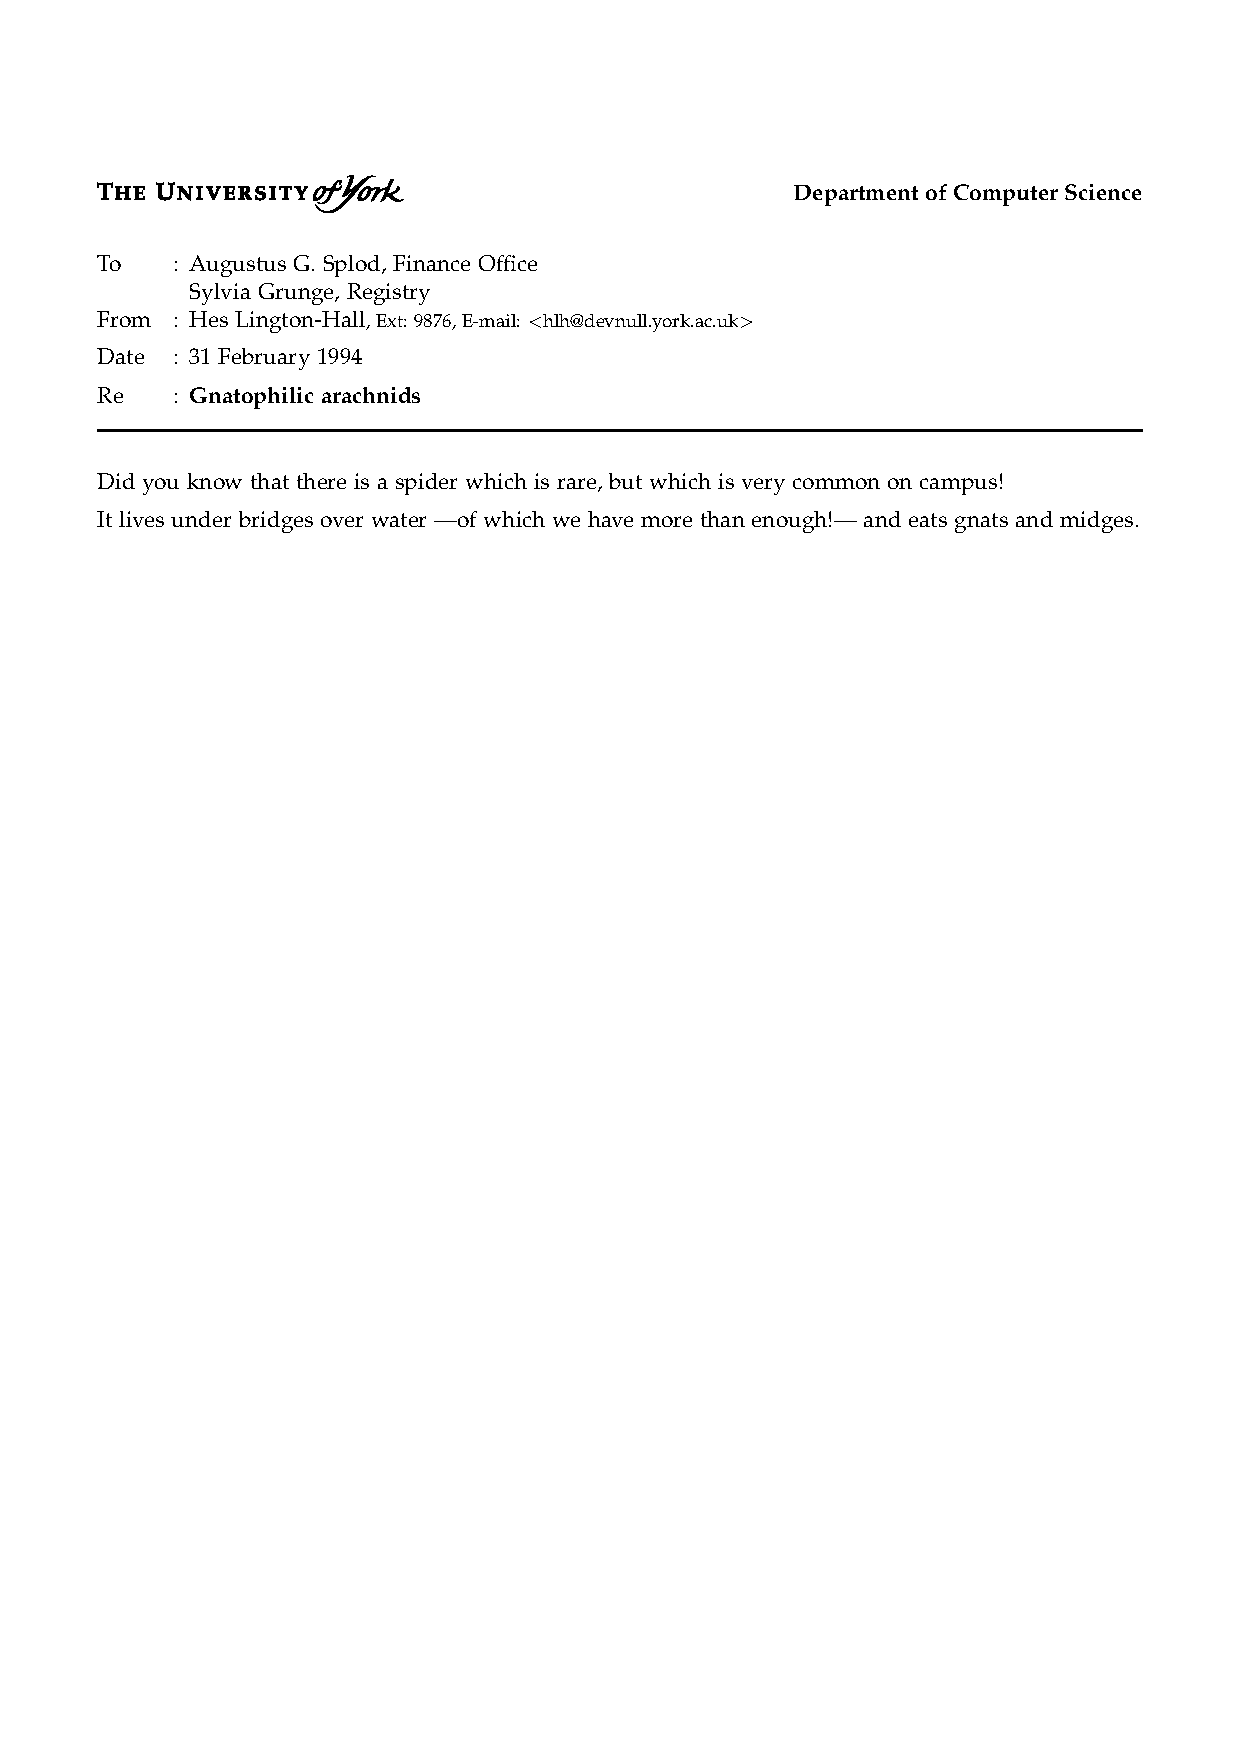
\includegraphics{Example}}}
\caption{The output from the file of Figure \protect\ref{Example1:Fig}}
\label{Output:Fig}
\end{figure}

\section{Making a personal memorandum class}

It is possible to save typing by creating your own sub-class of
\cmdsty{UoYmemo}.  By creating a file called \cmdsty{HLHmemo.cls}
with contents as in Figure \ref{Cls:Fig} the example in Figure
\ref{Example1:Fig} could have been typed as in Figure
\ref{Example2:Fig}.
\begin{figure}[p]
{\sffamily
\begin{tabular}[t]{l}
\pcmd{NeedsTeXFormat}{LaTeX2e}\\
\pcmd{ProvidesClass}{HLHmemo}[1994/09/13 Private Class for HLH]\\
\pcmd{DeclareOption*}
        {\pcmd{PassOptionsToClass}{\cmd{CurrentOption}}$\{$UoYmemo$\}$}\\
\cmd{ProcessOptions}\\
\pcmd{LoadClass}{UoYmemo}\\
\pcmd{from}{Hes Lington-Hall}\\
\pcmd{fromaddress}{Computer Science}\\
\pcmd{fromext}{6666}\\
\pcmd{fromemail}{hlh@devnull.york.ac.uk}\\
\end{tabular}
}
\caption{An example sub-class of \cmdsty{UoYmemo}}\label{Cls:Fig}
\end{figure}
\begin{figure}[p]
{\sffamily
\begin{tabular}[t]{l}
\pcmd{documentclass[12pt]}{HLHmemo}\\
\pcmd{date}{31 February 1944}\\
\pcmd{to}{Augustus G. Splod, Finance Office}\\
\pcmd{subject}{Gnatophilic arachnids}\\
\pcmd{begin}{document}\\
Did you know that there is a spider which is rare,\\
but which is very common on campus!\\
It lives under bridges over water ---of which we\\
have more than enough!--- and eats gnats and midges.\\
\pcmd{end}{document}
\end{tabular}
}
\caption{A memorandum made with the private class of
                Figure \protect\ref{Cls:Fig}.}
\label{Example2:Fig}
\end{figure}

See the Local Guide to find out how to persuade \LaTeX\ to take notice
of your personal memorandum class.

\section{Other packages and files used by \cmdsty{UoYmemo}}

Class \cmdsty{UoYmemo} loads the standard packages
\cmdsty{t1enc}, \cmdsty{palatino} and the local package
\cmdsty{UoYlogo}.  In turn \cmdsty{UoYlogo} loads \cmdsty{graphics}
and \cmdsty{color} (but the logo does not appear in colour yet!) and
needs a source for the University logo in PostScript (see the
documentation for \cmdsty{UoYlogo}).

\end{document}
